\documentclass{article}

\usepackage[left=2cm,right=2cm, top=2cm, bottom = 2cm]{geometry}
\usepackage{amsfonts}

\usepackage{amsmath}
\usepackage{xcolor}

\usepackage{tikz}
\usepackage{subfigure}



\pagestyle{empty}

\setlength{\tabcolsep}{15pt}







\begin{document}

\title{Determinants and Inverse Matrices}
\date{}

\maketitle
\thispagestyle{empty}

\Large

\textbf{\underline{Objective: To compute the determinants and inverses of $2\times 2$ and}}

\textbf{\underline{$3\times 3$ matrices.}}






\vspace{5mm}

\textbf{Warm-up:}\bigskip

Let $A$ be the matrix
\[A=\left(\begin{array}{cc} 3 & 0 \\ 1 & 2\end{array}\right)\]
and let $e_1$ and $e_2$ be the standard unit vectors:
\[e_1=\left(\begin{array}{c} 1 \\ 0 \end{array}\right),\quad e_2 = \left(\begin{array}{c} 0 \\ 1 \end{array}\right).\]

\begin{enumerate}
	\item Plot the points with position vectors $e_1$, $e_2$, and $e_1+e_2$.
	\item Compute $Ae_1$, $Ae_2$, and $A(e_1+e_2)$.
	\item Consider the unit square $S$, with vertices $(0,0)$, $e_1$, $e_2$, and $e_1+e_2$, and its image $A(S)$, with vertices $0$ and the three points found above. Find the area of $A(S)$.
	\item The determinant of a $2\times 2$ matrix
		\[\left(\begin{array}{cc}a&b\\c&d\end{array}\right)\]
		is given by $ad-bc$. Compute the determinant of $A$ and compare with your answer to part 3.
\end{enumerate}

\clearpage



\textbf{Theory: Matrices and Scale Factors:}\bigskip


With $e_1$ and $e_2$ the standard unit vectors as above, the unit square $S$ has vertices $(0,0)$, $e_1$, $e_2$, and $e_1+e_2$. If $A$ is the matrix
\[A=\left(\begin{array}{cc}a&b\\c&d\end{array}\right),\]
then when we apply $A$ to these points, we get $(0,0)$, $Ae_1=(a,c)$, $Ae_2=(b,d)$, and $A(e_1+e_2)=(a+b,c+d)$. These four points define a parallelogram $A(S)$ in the plane. The unit square has area 1, so the area of $A(S)$ can be thought of as a ``scale factor'' for $A$---it says how much $A$ has enlarged (or shrunk) the unit square by. In fact, this scale factor will tell us how much the area of any shape is changed by $A$.

\begin{center}
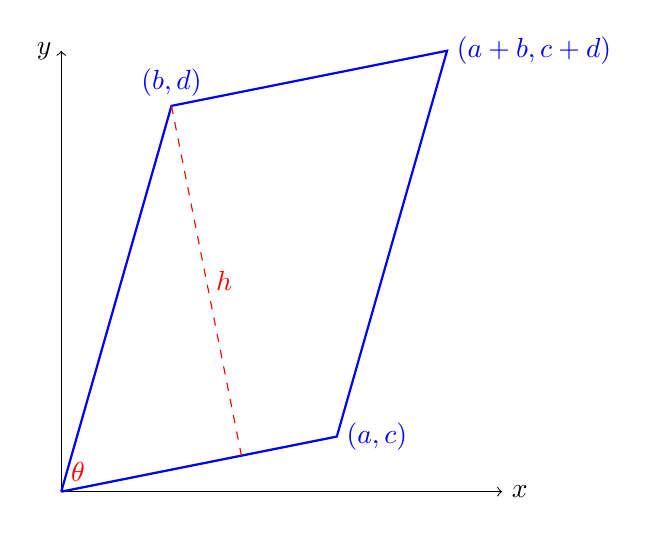
\begin{tikzpicture}[scale=0.7]
	\draw[->] (0,0) -- (8,0);
	\node[right] at (8,0) {$x$};
	\draw[->] (0,0) -- (0,8);
	\node[left] at (0,8) {$y$};
	
	\draw[thick,blue] (0,0) -- (5,1) -- (7,8) -- (2,7) -- (0,0);
	\node[right,blue] at (5,1) {$(a,c)$};
	\node[above,blue] at (2,7) {$(b,d)$};
	\node[right,blue] at (7,8) {$(a+b,c+d)$};
	
	\draw[red,dashed] (2,7) -- ({2+33/26},{7-165/26});
	\node[red,right] at ({2+33/52},{7-165/52}) {$h$};
	\node[red,above right] at (0,0) {$\theta$};
\end{tikzpicture}
\end{center}

The area of a parallelogram is the length of a side times the perpendicular height; there the area of the above parallelogram is $h\sqrt{a^2+c^2}$. By SohCahToa, $h=\sqrt{b^2+d^2}\sin(\theta)$. Since $\theta$ is the angle between the vectors $(a,c)$ and $(b,d)$, we have
\[(a,c)\cdot(b,d) = \sqrt{a^2+c^2}\sqrt{b^2+d^2}\cos(\theta).\]

Hence show that the area of the parallelogram is $ad-bc$.

\vfill


We have assumed in the above diagram that $a$, $b$, $c$, and $d$ are all positive. However, by checking all possiblities (rather tediously) we can confirm that $ad-bc$ always gives plus or minus the area of the parallelogram, and it gives the negative value precisely when the orientation is reversed---\textit{i.e.}, when $(a,c)$ makes a bigger angle with the positive $x$-axis than $(b,d)$ does.



\clearpage



\textbf{Determinants:}\bigskip

So we have shown that if
\[A=\left(\begin{array}{cc}a&b\\c&d\end{array}\right),\]
then the quantity $ad-bc$ is the scale factor by which the area of the unit square is enlarged when transformed by $A$, with a sign telling us about the orientation. This quantity is called the \textbf{determinant} of $A$ and written $\det(A)$ or $|A|$. The determinant doesn't contain enough information to tell us everything about $A$---after all, we can easily write down two different matrices with the same determinant---but it does give us a good idea of what $A$ does, in terms of both scale and orientation.

When writing determinants, we often drop the parentheses around matrices. For instance, we would write
\[\left|\begin{array}{cc}4&6\\-3&1\end{array}\right|\]
instead of
\[\left|\left(\begin{array}{cc}4&6\\-3&1\end{array}\right)\right|\]

\bigskip


\textbf{Practice:}\bigskip

\begin{enumerate}
	\item For each of the following matrices, find its determinant and state whether it is orientation-preserving or orientation-reversing.
		\begin{enumerate}
			\item $\left(\begin{array}{cc}4&6\\-3&1\end{array}\right)$.
			\item $\left(\begin{array}{cc}2&0\\7&3\end{array}\right)$.
			\item $\left(\begin{array}{cc}0&2\\7&3\end{array}\right)$.
		\end{enumerate}
	\item Calculate $\left|\begin{array}{cc}1&-3\\-4&12\end{array}\right|$. Interpret this result in terms of areas; what does it tell you about the transformation represented by the matrix?
\end{enumerate}



\clearpage



\textbf{Determinants of $3\times 3$ Matrices:}\bigskip

We have seen that the determinant of a $2\times 2$ matrix tells us how it affects area and orientation. A $3\times 3$ matrix acts naturally on 3-dimensional space, so instead of area we should consider how volume is affected. We can take the unit cube, defined by having $(0,0,0)$, $e_1=(1,0,0)$, $e_2=(0,1,0)$, $e_3=(0,0,1)$, $e_1+e_2$, $e_1+e_3$, $e_2+e_3$, and $e_1+e_2+e_3$ as vertices, transform it by a matrix $A$, and work out the volume of the resulting parallelepiped, similarly to how we did in the 2D case. However, this would be a very fiddly and tedious calculation, and would give us a complicated formula.

The formula for a $3\times 3$ determinant is complicated enough that nobody bothers to remember it. Instead, people remember a method for computing $3\times 3$ determinants in several steps. There are numerous such methods (and they also apply for larger $n\times n$ matrices); the one in the A-level Further Maths syllabus is called \textbf{Laplace expansion}. To describe the method, we need a number of definitions; unfortunately, there's a lot of terminology here, but the method is more important than the names of all the parts!\medskip


In an $n\times n$ matrix $A$, the $(i,j)$\textbf{-minor} of $A$ is the determinant of the $(n-1)\times(n-1)$ matrix made by deleting the $i^\mathrm{th}$ row and $j^\mathrm{th}$ column of $A$. The matrix formed by replacing every element of $A$ by its minor is called the \textbf{matrix of minors} of $A$. An example will illustrate:\medskip

Compute the matrix of minors for $\left(\begin{array}{ccc}1&0&2\\7&3&-1\\9&-2&0\end{array}\right)$.



\clearpage



\textbf{Determinants of $3\times 3$ Matrices (cont.):}\bigskip


Given an $n\times n$ matrix $A$, the determinant $|A|$ is found by taking any row or column, multiplying each entry in that row or column by its minor, and then adding them up according to the \textbf{rule of alternating signs}, which says that you start with $+$ in the top-left, and alternate between $+$ and $-$ as you move rows or columns. In the $3\times 3$ case, the rule of alternating signs is illustrated by the diagram
\[\left(\begin{array}{ccc}+&-&+\\-&+&-\\+&-&+\end{array}\right).\]

\bigskip


We found the matrix of minors of
\[\left(\begin{array}{ccc}1&0&2\\7&3&-1\\9&-2&0\end{array}\right)\]
on the last page; now we will find its determinant. We can expand along any row or column, and will try several to show they all give the same answer.

\vfill


Note that we do not need to know the entire matrix of minors to find the determinant---just one row or one column of it. We usually write down the determinant calculation as follows:\medskip

Find $\left|\begin{array}{ccc}-3&0&12\\-3&3&8\\7&0&4\end{array}\right|$.

\clearpage






\textbf{Practice:}\bigskip



\begin{enumerate}
	\item For each of the following matrices, find its determinant and state whether it is orientation-preserving or orientation-reversing.
		\begin{enumerate}
			\item $\left(\begin{array}{ccc}4&3&6\\2&1&-7\\5&8&4\end{array}\right)$.
			\item $\left(\begin{array}{ccc}0&4&0\\0&0&-3\\5&0&0\end{array}\right)$.
		\end{enumerate}
	\item Calculate $\left|\begin{array}{ccc}100&0&0\\0&300&0\\30&90&0\end{array}\right|$. Interpret this result in terms of volumes; what does it tell you about the transformation represented by the matrix?
	\item For what values of $a$ is the determinant of the following matrix 0?
		\[\left(\begin{array}{ccc}a&4&0\\3&a+1&-3\\1&0&a\end{array}\right).\]
	\item Calculate the matrix of minors of $\left(\begin{array}{cc}a&b\\c&d\end{array}\right)$. Hence use Laplace expansion to find the determinant, and compare with the formula we used before.
	\item Bonus question: calculate the $4\times 4$ determinant
		\[\left|\begin{array}{cccc}1&3&0&-2\\4&7&-6&9\\0&3&-6&3\\-5&-13&12&-10\end{array}\right|.\]
		You should get 0. Note: you do not need to calculate $4\times 4$ determinants at A-level; if you can do it, you should have no problem with any determinant they ask you.
\end{enumerate}



\clearpage


\textbf{Inverse Matrices:}\bigskip

An $n\times n$ matrix represents a transformation of $n$-dimensional space. Can we undo the transformation? For instance,
\[R_\theta=\left(\begin{array}{cc} \cos(\theta)&-\sin(\theta)\\\sin(\theta)&\cos(\theta)\end{array}\right)\]
represents a rotation by an angle $\theta$ anticlockwise about the origin. Rotation by $-\theta$ should return us to where we started, and is given by
\[R_{-\theta}=\left(\begin{array}{cc} \cos(-\theta)&-\sin(-\theta)\\\sin(-\theta)&\cos(-\theta)\end{array}\right)=\left(\begin{array}{cc} \cos(\theta)&\sin(\theta)\\-\sin(\theta)&\cos(\theta)\end{array}\right).\]

So we should have $R_\theta R_{-\theta}=I_2$, the $2\times 2$ identity matrix. Verify this.

\vfill


Let $A$ be a general $2\times 2$ matrix:
\[A=\left(\begin{array}{cc}a&b\\c&d\end{array}\right).\]
Form the matrix of minors of $A$, apply the rule of alternating signs to it, and take the transpose. The resulting matrix is called the \textbf{adjugate matrix} of $A$. Multiply $A$ by its adjugate matrix (in both orders).

\vfill

\clearpage



\textbf{Inverse Matrices (cont.):}\bigskip

We saw on the last page that if $A$ is a $2\times 2$ matrix and $\mathrm{adj}$ is its adjugate matrix, then
\[A\cdot \mathrm{adj}(A)=\mathrm{adj}(A)\cdot A=|A|I_2.\]
This is the $2\times 2$ case of a result called \textbf{Cramer's rule}. Therefore, if we let $A^{-1}=\frac{1}{|A|}\mathrm{adj}(A)$, we have
\[AA^{-1}=A^{-1}A=I_2,\]
so $A^{-1}$ is inverse to $A$.

This gives us a formula for the inverse of a $2\times 2$ matrix:
\[\left(\begin{array}{cc}a&b\\c&d\end{array}\right)^{-1}=\frac{1}{ad-bc}\left(\begin{array}{cc}d&-b\\-c&a\end{array}\right).\]\bigskip


Generalising to higher dimensions, Cramer's rule says that if we take an $n\times n$ matrix $A$, take its matrix of minors, apply the rule of alternating signs (to form the \textbf{matrix of cofactors}), then transpose, we get the adjugate matrix $\mathrm{adj}(A)$, and then
\[A^{-1}=\frac{1}{|A|}\mathrm{adj}(A).\]\bigskip

Find the inverse of $\left(\begin{array}{ccc}1&0&2\\7&3&-1\\9&-2&0\end{array}\right)$.

\clearpage


\textbf{Further Theory:}\bigskip


We have seen that to find the inverse of a matrix, we must divide the adjugate matrix by the determinant. What if the determinant is 0? In this case, no inverse matrix exists; geometrically, a matrix with inverse determinant must collapse at least one dimension down to nothing---think of our examples with $2\times 2$ and $3\times 3$ determinants---so it must lose information, and so we cannot recover what we started with.\bigskip

We have only considered square matrices; can a non-square matrix have an inverse? The answer is no, but it can have a ``one-sided'' inverse:
\[\left(\begin{array}{ccc} 1 & 0 & 0\\ 0 & 1 & 0\end{array}\right)\cdot \left(\begin{array}{cc} 1 & 0\\ 0 & 1\\ 0 & 0\end{array}\right)=\]

\[\left(\begin{array}{cc} 1 & 0\\ 0 & 1\\ 0 & 0\end{array}\right)\cdot \left(\begin{array}{ccc} 1 & 0 & 0\\ 0 & 1 & 0\end{array}\right)=\]

This raises a worrying possibility: suppose $A$ and $B$ are $n\times n$ matrices and $AB=I_n$; it seems like $BA$ could fail to be $I_n$. In fact, this cannot occur: with square matrices, if they are inverse one way round, they are the other two; proving this requires a powerful result called the Rank-Nullity Theorem and is well beyond A-level.

\clearpage


\textbf{Practice:}\bigskip

Find the inverses of the following matrices:

\begin{enumerate}
	\item $\left(\begin{array}{cc}4&6\\-3&1\end{array}\right)$.
	\item $\left(\begin{array}{cc}2&0\\7&3\end{array}\right)$.
	\item $\left(\begin{array}{cc}0&2\\7&3\end{array}\right)$.
	\item $\left(\begin{array}{ccc}4&3&6\\2&1&-7\\5&8&4\end{array}\right)$.
	\item $\left(\begin{array}{ccc}0&4&0\\0&0&-3\\5&0&0\end{array}\right)$.
	\item $\left(\begin{array}{cccc}3&0&4&0\\1&0&-3&0\\5&0&0&-2\\0&1&1&0\end{array}\right)$.
	
		Note: finding inverses of $4\times 4$ matrices is beyond A-level.
\end{enumerate}



\end{document}